\documentclass[a4paper]{report}

\usepackage[english]{babel}
\usepackage{caption}
\usepackage{subcaption}
\usepackage{listings, color}
\usepackage{graphicx}
\usepackage{chngpage}
\usepackage{longtable}
\usepackage{float}
\usepackage{comment}
\usepackage[usenames,dvipsnames]{xcolor}
\usepackage{epstopdf}
\usepackage{titlesec}
\usepackage{pdfpages}
\usepackage{wrapfig}
\usepackage{url}
\usepackage{hyperref}
\usepackage[nodisplayskipstretch]{setspace}
\usepackage[top=2cm,bottom=2.5cm]{geometry}
\usepackage{amsmath}
\usepackage{caption} 
\usepackage{natbib}
\usepackage[nottoc,numbib]{tocbibind}
\usepackage{xpatch}

\definecolor{dkgreen}{rgb}{0,0.6,0}
\definecolor{gray}{rgb}{0.5,0.5,0.5}
\definecolor{mauve}{rgb}{0.58,0,0.82}

\lstset{frame=tb,
  language=Matlab,
  aboveskip=3mm,
  belowskip=3mm,
  showstringspaces=false,
  columns=flexible,
  basicstyle={\small\ttfamily},
  numbers=left,
  numberstyle=\tiny\color{gray},
  keywordstyle=\color{black},
  commentstyle=\color{dkgreen},
  stringstyle=\color{mauve},
  breaklines=true,
  breakatwhitespace=true
  tabsize=3
}

\newcommand{\tab}{\hspace*{2em}}
\titleformat{\chapter}{\normalfont\huge\bf}{\thechapter.}{20pt}{\huge\bf}

\newcommand\fnurl[2]{%
  \href{#2}{#1}\footnote{\url{#2}}%
}


\xpatchcmd{\itemize}
  {\def\makelabel}
  {\setlength{\itemsep}{0em}\def\makelabel}
  {}
  {}

\begin{document} 
\begin{titlepage}

\newcommand{\HRule}{\rule{\linewidth}{0.5mm}} % Defines a new command for the horizontal lines, change thickness here

\center % Center everything on the page
 
%----------------------------------------------------------------------------------------
%	HEADING SECTIONS
%----------------------------------------------------------------------------------------

\textsc{\LARGE Group 7}\\[1.5cm] % Name of your university/college

%----------------------------------------------------------------------------------------
%	TITLE SECTION
%----------------------------------------------------------------------------------------

\HRule \\[0.4cm]
{ \huge \bfseries Assignment 3}\\[0.4cm] % Title of your document
\HRule \\[4cm]
 
%----------------------------------------------------------------------------------------
%	AUTHOR SECTION
%----------------------------------------------------------------------------------------

\begin{minipage}{0.5\textwidth}
\emph{Authors:}\\     
Emilie de Bree - 4247558\\
Toine Hartman - 4305655\\
Jeffrey Helgers - 4318749 \\
Jim Hommes - 4306090\\
Joost Pluim - 4162269 \\
Matthijs Verzijl - 4282604\\\\
\emph{Supervisor:} \\
Alberto Bacchelli \\\\
\emph{Teaching Assistant:} \\
Aaron Ang\\
\end{minipage}\\[4cm]


%----------------------------------------------------------------------------------------
%	LOGO SECTION
%----------------------------------------------------------------------------------------


\includegraphics[width=100mm]{logo.jpg}\\[1cm] % Include a department/university logo - this will require the graphicx package

%----------------------------------------------------------------------------------------
%	DATE SECTION
%----------------------------------------------------------------------------------------

{\large \today}\\[3cm] % Date, change the \today to a set date if you want to be precise

\vfill % Fill the rest of the page with whitespace

\end{titlepage}
\tableofcontents
\thispagestyle{empty}
\setcounter{page}{0}
\chapter{Resonsibility Driven Design}
Here the features of Respsonsibility Driven Design will be explained per feature we added this sprint.

\section{Jumping on Bubbles}
\subsubsection{Player}
\textit{Responsibility:}  \\
The player class will handle the movement of the player. \\
\textit{Collaborations:} \\
It will be communicating with SpriteBase for collisions. \\

\subsubsection{SpriteBase}
\textit{Responsibility:}  \\
SpriteBase will be responsible for detecting collisions with BubbleSprites. \\
\textit{Collaborations:} \\
It will be communicating with Player. \\

\section{Warping}
\subsubsection{Level}
\textit{Responsibility:}  \\
When loading the map, it should be clear where the player is able to warp. \\
\textit{Collaborations:} \\
When the player collides with a warpable area, Level should communicate with Player to tell him where he warped to. \\

\subsubsection{Player}
\textit{Responsibility:}  \\
This class will be moving the player and spawning it after the warp. \\
\textit{Collaborations:} \\
When the player warped, it communicates with ScreenController to be redrawn. \\

\section{Refactoring Controllers for Testing}
\subsubsection{LevelController}
\textit{Responsibility:}  \\
The responsibility for this class will \textit{only} include creating levels and all communication between the objects in the game. \\
\textit{Collaborations:} \\
It will communicate with the objects in de game (Model package) and with the MainController. It will also be the bridge to ScreenController for the SpriteBases. \\

\subsubsection{MainController}
\textit{Responsibility:}  \\
MainController will be the controller that is loaded by the FXML. It will have all untestable objects and will seperate the GUI from the LevelController. \\
\textit{Collaborations:} \\
LevelController and ScreenController will communicate via MainController. \\

\section{Better Physics}
\subsubsection{Player}
\textit{Responsibility:}  \\
Player is responsible for the movement of the player itself. \\
\textit{Collaborations:} \\
Player will be communicating with LevelController for the set of walls it could collide with. This all affects the physics. \\
\chapter{Updated UML}
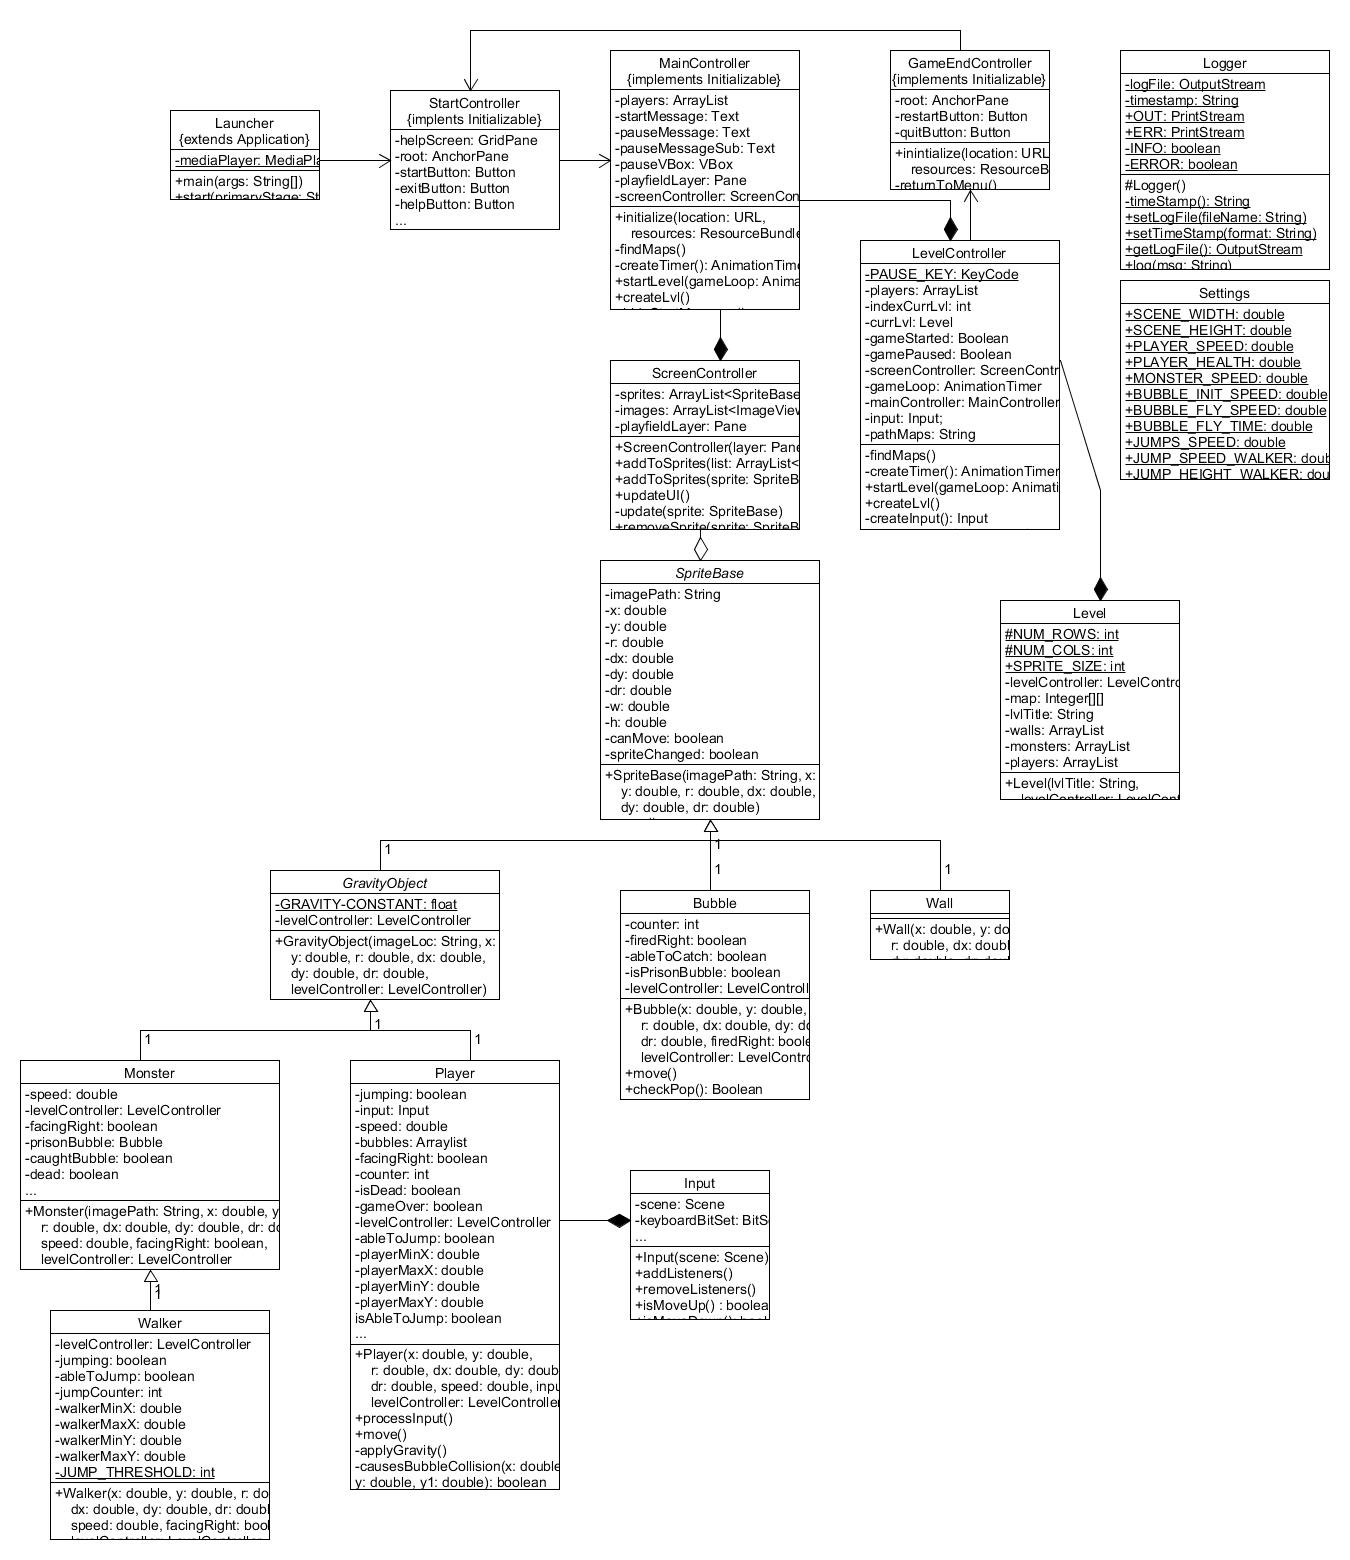
\includegraphics[width=160mm]{classDiagramsUML_3.jpg}
%Your text files go here
\nocite{*}
\bibliographystyle{newapa}
\end{document}